\chapter{The CMS Detector}
\label{chap:detector}

To ensure as much as possible of the debris of the proton-proton collisions can be detected, CMS is constructed to maximize the solid-angle coverage of the interaction region. It is a modular design of subsystems, each with its own technology specialized for detection of specific types of particles. In fact, among all the known particles to exist there are only a handful which are stable enough to interact within our detector: electrons $e^{\pm}$, muons $\mu^{\pm}$, pions $\pi^{\pm}\,\pi^{0}$, photons $\gamma$, neutrons n, protons $p^{\pm}$, and kaons $K^{\pm}\,K^{0}$. Neutrinos $\nu$ do not interact at all within our detector and create an imbalance in the total momentum of the event. Many of the SM particles are unstable and have very short lifetimes causing them to decay to lighter particles (e.g. the list above) before they travel any appreciable distance in our detector. Figure \ref{fig:detectoreta} illustrates the and barrel ($|\eta|<1.5$) and endcap ($1.5<|\eta|<5$) regions, the beamline is seen as the thin cyan line across the base of the image. The beampipe physically limits the detector extending past $|\eta|>5$.

This chapter will discuss the main elements of the CMS detector, beginning with the innermost (closest to the beam pipe) silicon tracker and concluding with the muon tracker. An attempt will be made to succinctly detail the purpose the subdetector serves for the experiment, its operation principles, and geometrical form.

\begin{figure}[hbp!]
\centering
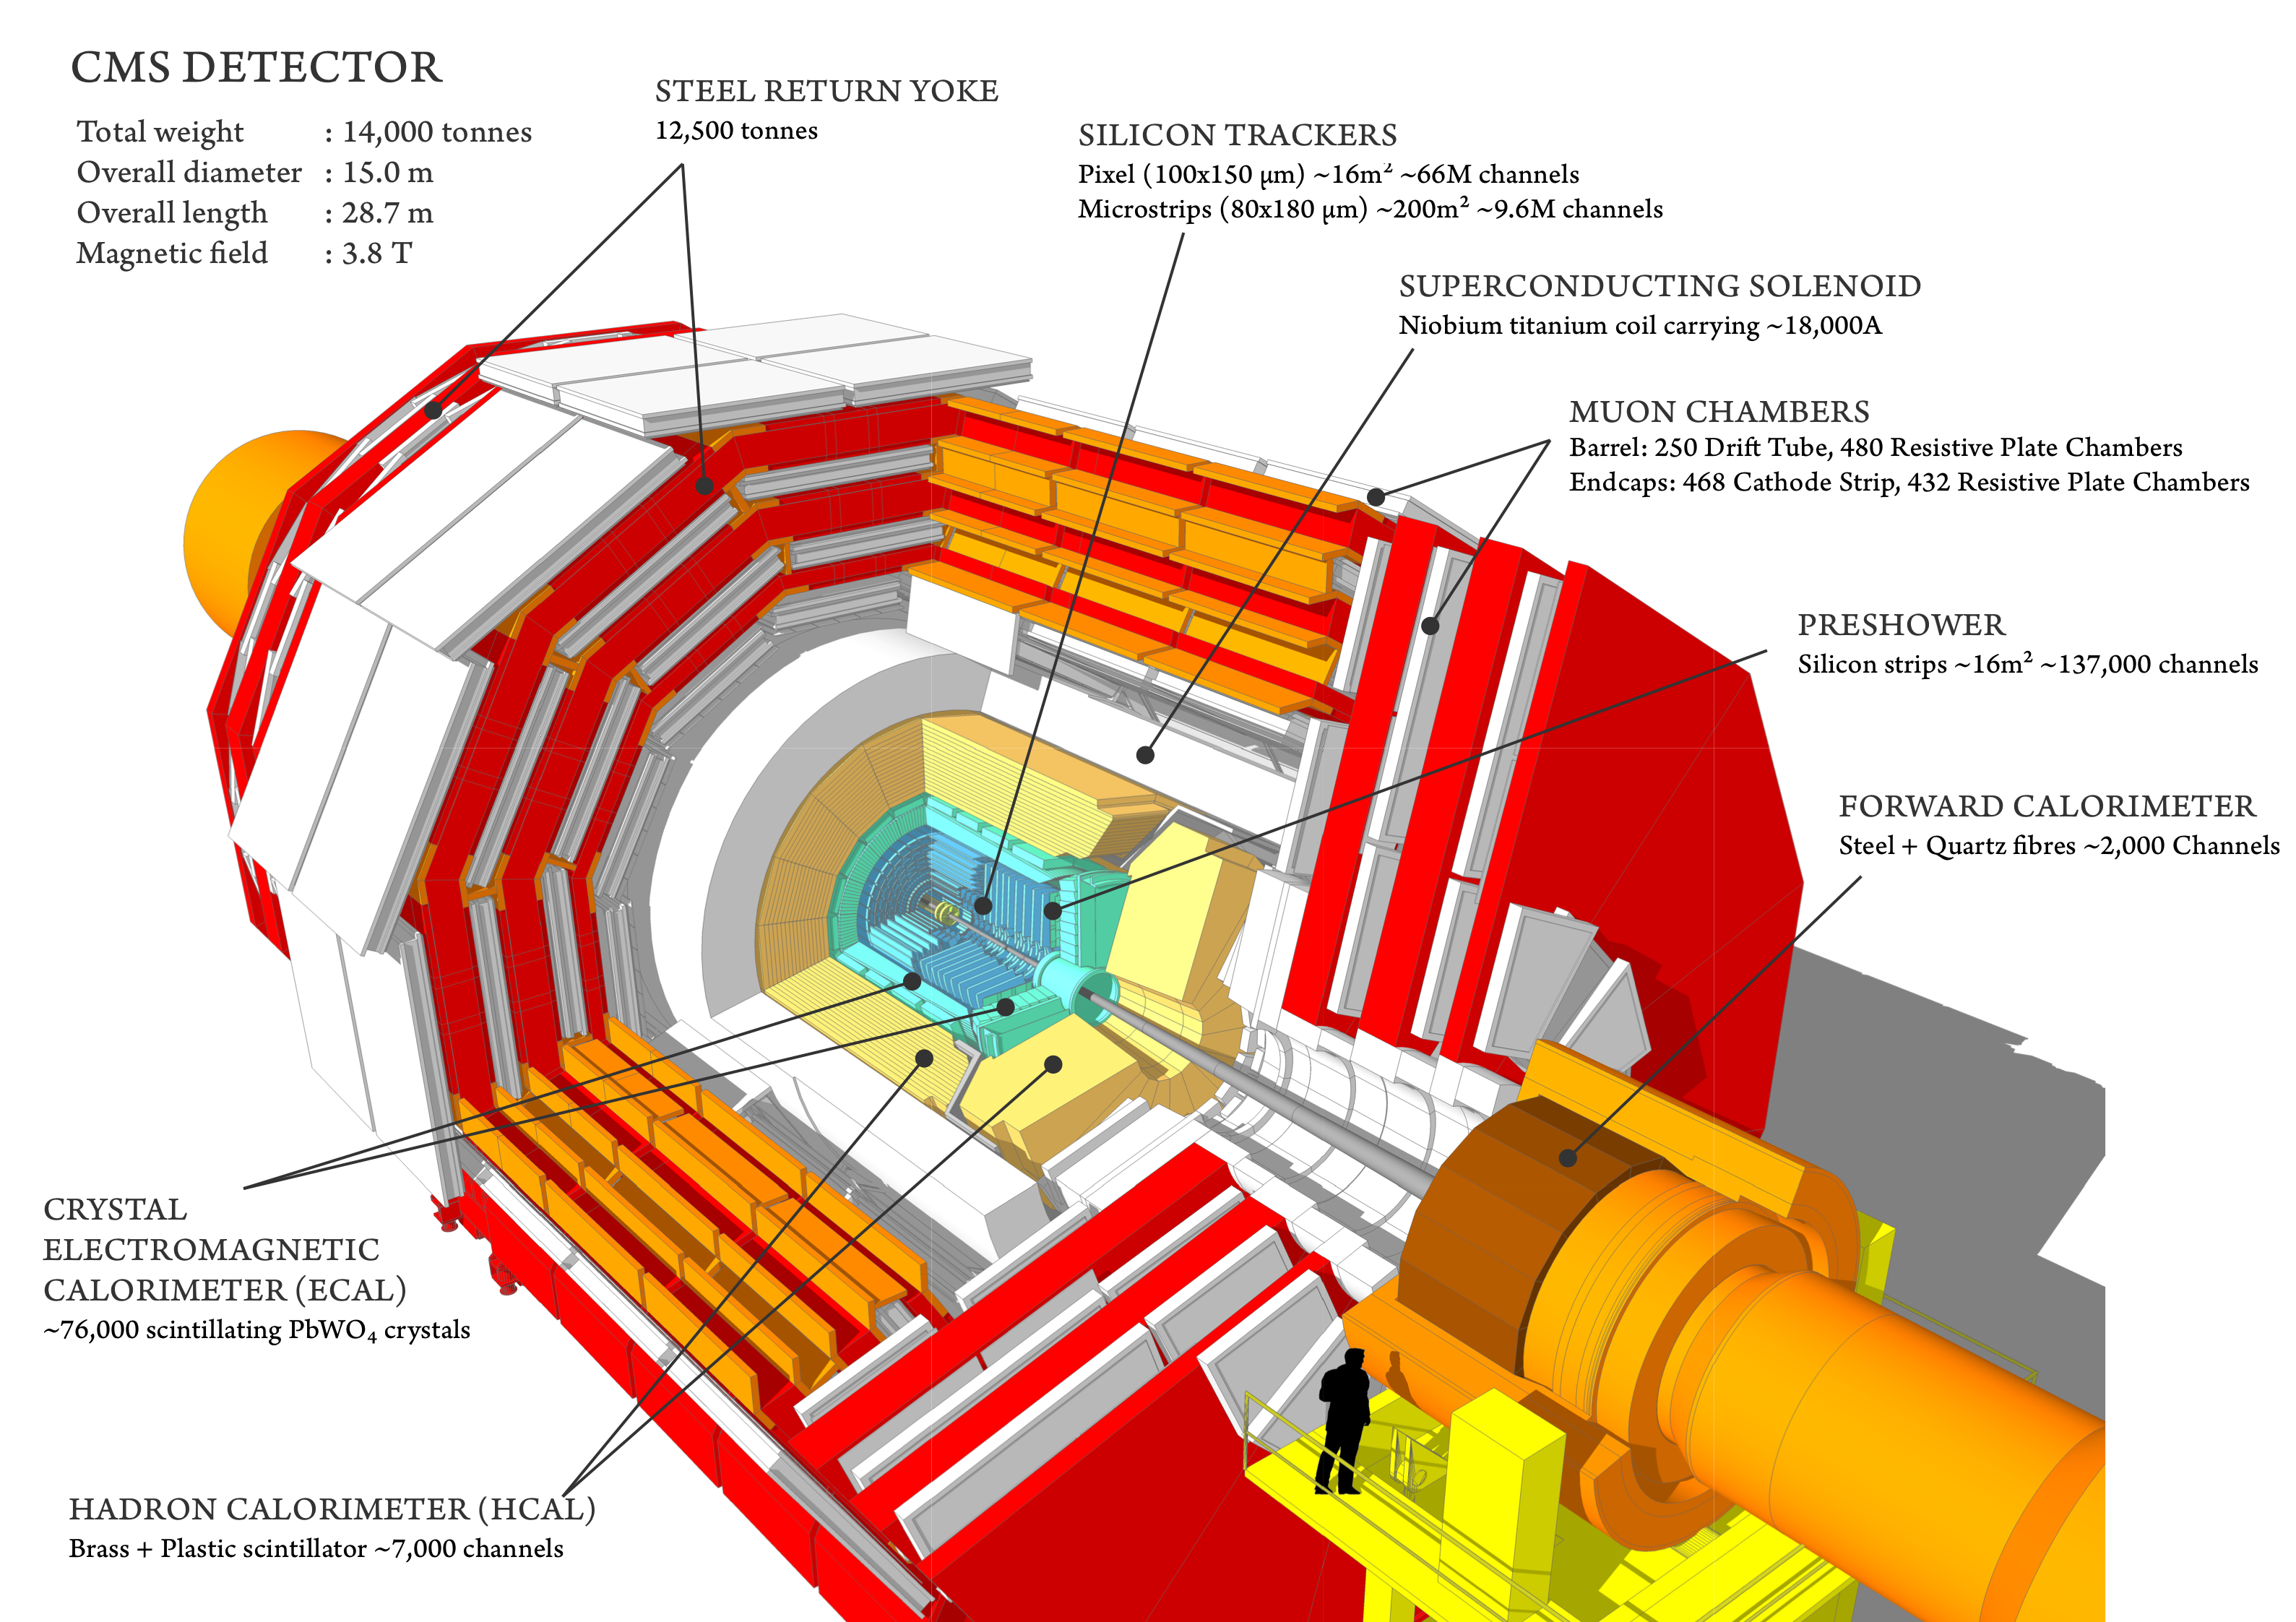
\includegraphics[width=0.9\textwidth]{figs/howcmsworks.png}
\caption{A view of the CMS detector.}
\label{fig:howcmsworks}
\end{figure}

\begin{figure}[hbp!]
\centering
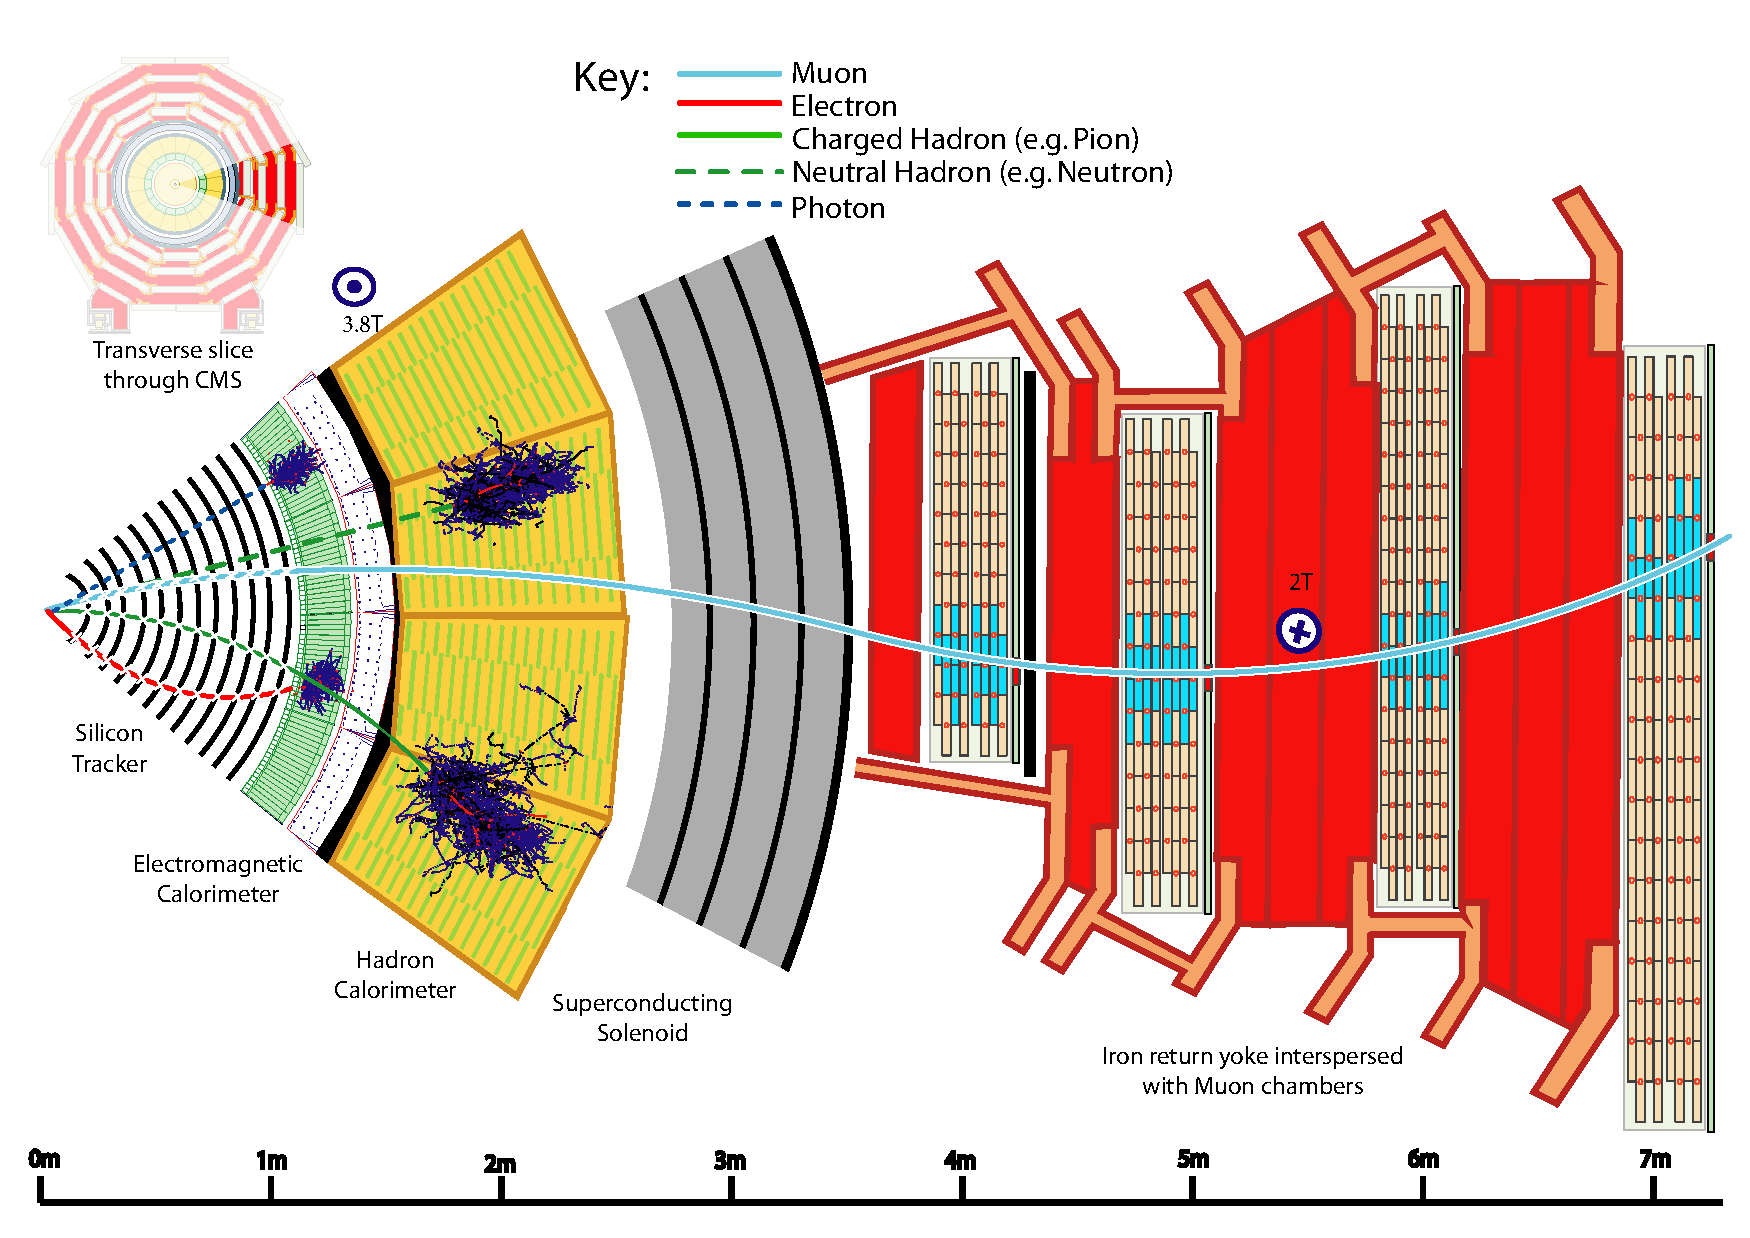
\includegraphics[width=0.7\textwidth]{figs/CMS-PRF-14-001_Figure_001.pdf}
\caption{A view of the CMS detector in the r-$\phi$ plane, in the barrel region of the detector.}
\label{fig:schematicview}
\end{figure}

\begin{figure}[hbp!]
\centering
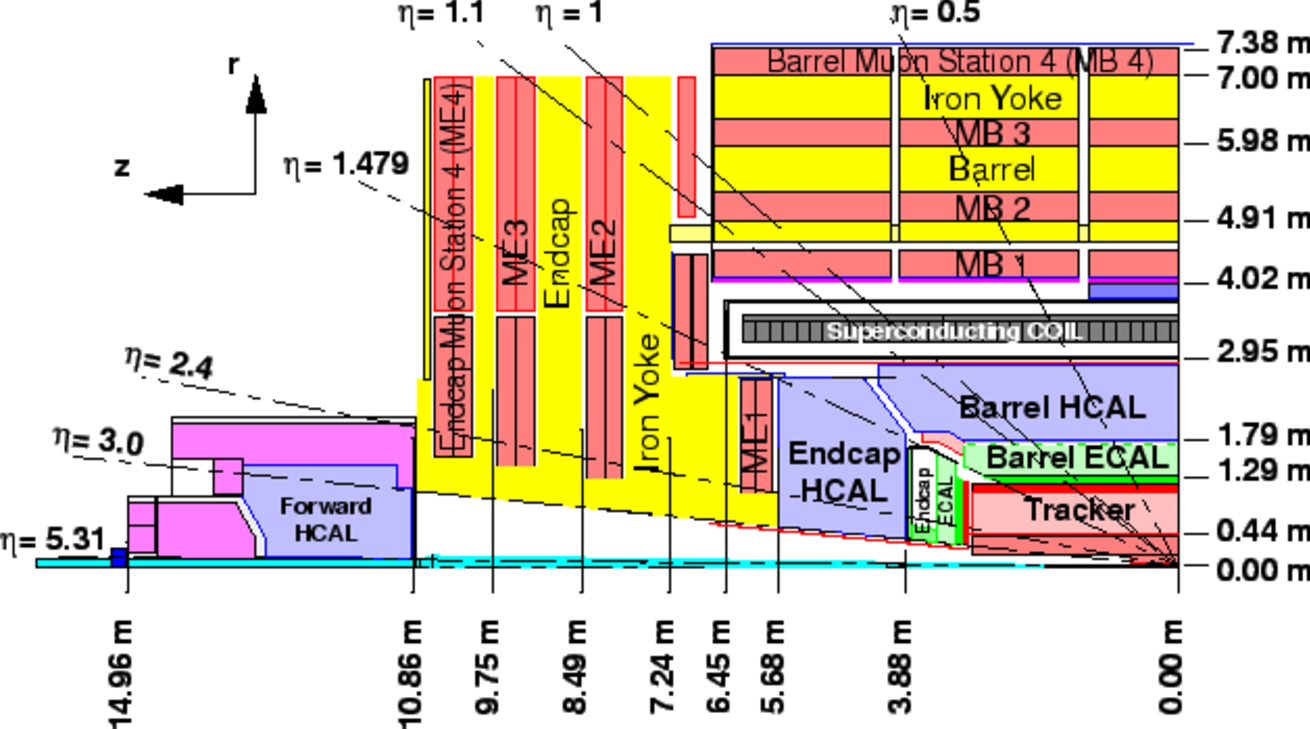
\includegraphics[width=0.8\textwidth]{figs/img41.pdf}
\caption{A view of the CMS detector in the r-z plane.}
\label{fig:detectoreta}
\end{figure}

\section{Silicon Tracker}

The silicon tracker is responsible for the reconstruction of charged particles: electrons, muons, kaons and pions. The particle trajectory is reconstructed using ionization deposits left in layers of thin silicon. The particle momentum is measured by the curvature of the trajectory when submerged in the magnetic field.\cite{trackertdr} \cite{trackertdradd}

The tracker is built of modules consisting of a reversed-biased, fully-depleted, silicon p-n junction. As a charged particle travels through the material, it ionizes the silicon creating electron-hole pairs within the depletion zone. Electric fields accelerate the charge through the silicon and to the readout electronics bonded to the back of the sensor where the signal is then amplified and digitized, before being piped outside the detector. The silicon is very thin (~300$\mu$m), the tracker is constructed of as little material as possible so as not to perturb the original trajectory of the particle.

The silicon tracker is divided into two major components. The pixel detector is at a closer proximity to the beam line and has finer spatial segmentation. The strips detector covers a larger spatial volume and is responsible for the majority of the hits along a particle trajectory.

\subsection{Pixel Detector}

The task of the pixel detector is to provide the spatial granularity required for precision track vertexing (importance will be discussed in Chapter \ref{chap:eventreco}). The barrel region ($|\eta|<1.5$) of the pixel detector consists of 4 concentric cylinders sitting at radii between 2.9 and 16 cm from the beamline. The endcaps ($1.5<|\eta|<2.5$) consist of three discs on each side ($\pm$z) placed in between z = 3.2 and 4.8cm. The silicon modules are pixelated into elements $100x150\mu\,m$ wide, yielding more than 65 million individual readout channels.

\subsection{Strips Detector}

The silicon strips sit immediately outside the pixel detector and provides additional hits along a particle's trajectory: the barrel region ($|\eta|<1.5$) provides 10 layers, the endcaps ($1.5<|\eta|<2.5$) provide 12. The silicon modules are partitioned in strips ranging from $80-180\,\mu$m wide, yielding more than 10 million individual readout channels.

\section{Electromagnetic Calorimeter}

The electromagnetic calorimeter is responsible for the reconstruction of electrons $e^{\pm}$, photons $\gamma$ and charged pions $\pi^{\pm}$. The energy is measured by collecting the light generated by an electromagnetic shower as the particle is absorbed in the calorimeter.\cite{ecaltdr}\cite{ecaltdradd}

The bulk of the calorimeter consists of lead-tungstate (PbWO$_{4}$) crystal. Electromagnetic showers are created when high energy particle enters the material. Low-mass particles, such as electrons, scatter as they traverse the material and emit bremstrallung radiation in the form of lower-energy photons. Photons interact with the material and convert into an electron-positron pair, which themselves are able to then emit radiation. The light generated by this shower is collected using photodetectors mounted at the end of each crystal. Light incident on the photodetector first encounters silicon where the photon knocks an electron of a silicon atom. This electron is accelerated with an electric field onto an electrode surface which liberates electrons via the photoelectric effect. These electrons are accelerated onto another electrode which in turn liberate more electrons. This signal is then further amplified and digitized.

The electromagnetic calorimeter is divided into barrel ($|\eta|<1.5$) and endcap ($1.5<|\eta|<3$) regions comprising over 75,000 crystals. The crystals measure 2.2$\,$x$\,$2.2$\,$x$\,$23$\,$cm in the barrel (matching the Moliere radius of PbWO$_{4}$ - 2.2 cm) and 3$\,$x$\,$3$\,$x$\,$22$\,$cm in the endcaps; they are oriented radially outward from the interaction region. This thickness of absorber is sufficient to contain over 98\% of the energy of incident particles. Additionally, the electromagnetic calorimeter serves as an absorber for the hadronic calorimeter, initiating a shower in approximately 1/3 the particles headed for the hadronic calorimeter.

\subsection{Preshower}

The Preshower is a more finely segmented region of the electromagnetic calorimeter intended for greater spatial resolution for resolving electromagnetic showers. It consists of two alternating layers of lead absorber and Si detectors (like the tracker) which are able to reconstruct the electron-positron pairs created at an early stage in the showering process. The silicon detector is able to reconstruct the electron and positron trajectories allowing for the greater spatial resolution compared to the rest of the calorimeter.

The motivation for the Preshower is for the proper identification of high-$p_{T}$ neutral pion decay (98.8\% branching fraction to two photons). The Preshower only exists in a forward region $1.7<\eta<2.6$ where this poses the greatest challenge because of the pion kinematics.

\section{Hadronic Calorimeter}

The hadronic calorimeter is responsible for the reconstruction of hadrons: charged pions $\pi^{\pm}$, protons $p^{\pm}$, neutrons n, and kaons $K^{\pm}, K^{0}$. The particle energy is measured by collecting light generated by a hadronic shower as the particle is absorbed in the calorimeter.\cite{hcaltdr}

The bulk of the calorimeter consists of steel and brass absorber. A particle will interact with the material causing a shower of a number of secondary particles. These secondary particles in turn interact and this process creates a particle shower within the detector. Interspaced with the absorber are tiles of clear plastic scintillator which create flashes of light after de-excitation of the scintillating molecules embedded in the plastic. Fibers are ran throughout the plastic and absorb the light, which is then piped to hybrid photodiodes. Light incident on the photodiodes liberates electrons via the photoelectric effect which are then accelerated onto the surface of a silicon diode which further amplifies and digitizes the signal.

The hadronic calorimeter is divided into barrel ($|\eta|<1.2$), endcap ($1.2<|\eta|<3$), and forward regions ($1.2<|\eta|<3$) and contains over 9000 readout channels. In all regions the absorber is over a meter thick and consists of many layers of plates about 5cm thick. The scintillator plates are about 1cm thick. This thickness of absorber is sufficient to contain over 98\% of the energy of incident particles. There is an additional section of calorimeter in the barrel region which sits outside the magnet solenoid and detects late-starting showers.

\section{Solenoidal Magnet}

The CMS magnet provides the field necessary to deflect charged particles within the trackers to allow for a measurement of the momentum. The superconducting iron electromagnet delivers a uniform 3.8 T solenoidal field (parallel to the beampipe) within the silicon tracker volume. The magnetic field lines are returned via steel yokes sitting outside the magnet interspaced within the muon tracker volume, the field strength throughout the muon system is approximately 2 T. \cite{magnettdr}.

\section{Muon System}

The muon system is responsible for the reconstruction (and triggering) of muons $\mu^{\pm}$. The muon trajectory is reconstructed using ionization deposits left in layers of gaseous detectors. The muon momentum is measured by the curvature of the trajectory when submerged in the magnetic field.\cite{muontdr}

The muon detectors sit at the furthest distance from the beamline, and any particles which have made the journey traveled through many layers of detector material (e.g. silicon Si, lead tungstate PbWO$_{4}$, brass (Cu), iron Fe) before being detected. Because of the relatively long lifetime and large mass of the muon they are the only particles which are expected to reach the muon detectors.

There are three components of the muon detector: drift tubes, cathode strip chambers, and resistive plate chambers. The drift tubes and cathode strip chambers are primarily used for tracking in the barrel endcap regions, respectively. There is a small amount of overlap in coverage of the two subdetectors. The resistive plate chambers are used primarily for triggering and has coverage in the barrel and endcap regions, instrumented within the dritft tbins and cathode strip chambers.

\subsection{Drift Tubes}

The drift tubes are used for muon tracking in the barrel portion of the detector ($|\eta|<1.3$). The basic element is a gas tube 4$\,$x$\,$1.3$\,$cm in transverse size and 2$\,$-$\,$4$\,$m long (depending on its position). High-voltage is applied to a wire strung the length of the cylinder and collects charge released when an incident muon ionizes the gas mixture. For economic and safety reasons the gas mixture is chosen to be Ar and CO$_{2}$. An 85/15\% fraction is chosen for nice gas quenching (shower avalanche) and drift velocity properties. \cite{dtperformance}

The drift tubes are divided into four barrel regions (each called a station) at different radii within the magnetic return yoke. Each station contains 3 \textit{superlayers}, where a superlayer is composed of four layers of stacked tubes, each layer staggered by one half width. For each station, two of the superlayers are oriented parallel to the beamline for $r-\phi$ measurements and one superlayer is perpendicular to the beamline to allow for measurements of the r-z position. An image of a DT station is seen in Figure \ref{fig:superlayer}.

\begin{figure}[hbp!]
\centering
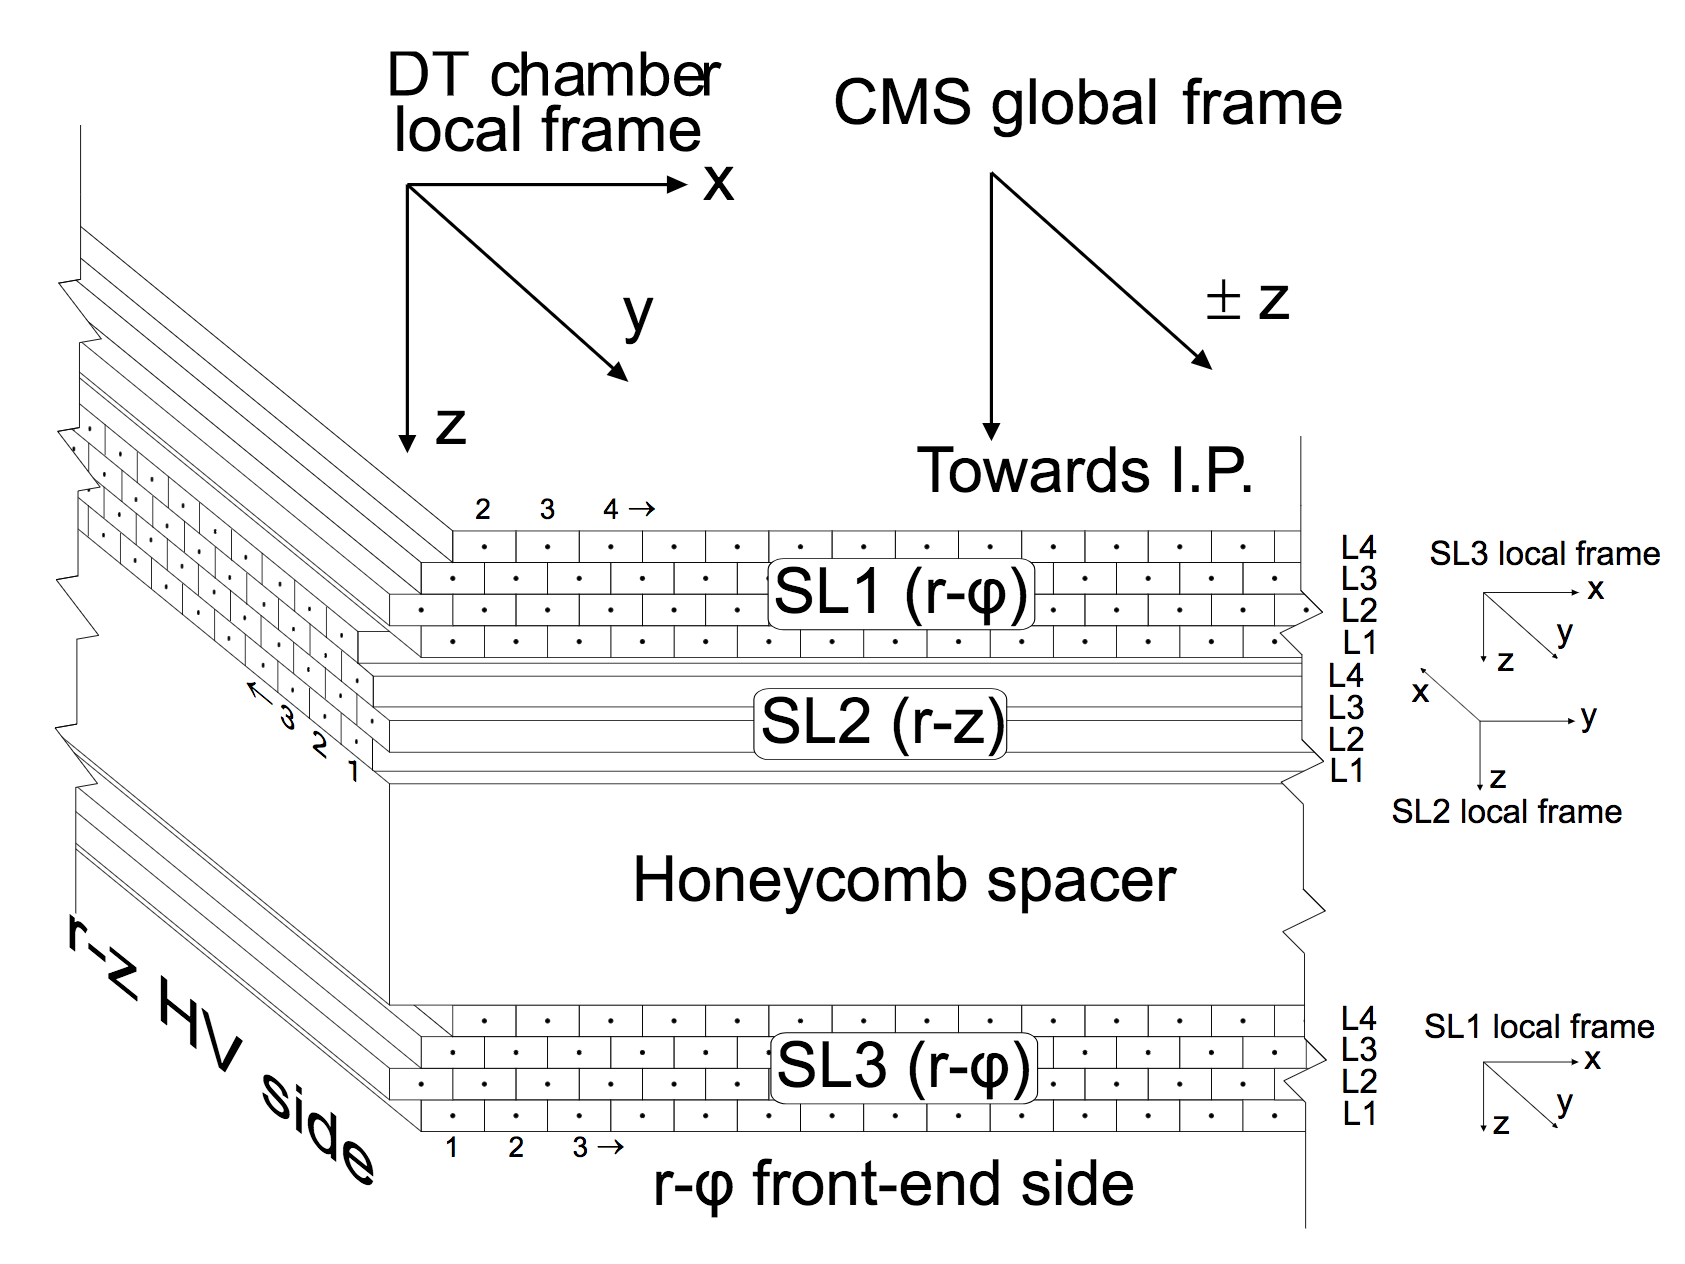
\includegraphics[width=0.65\textwidth]{figs/superlayer.png}
\caption{A diagram of a drift tube station.}
\label{fig:superlayer}
\end{figure}

\subsection{Cathode Strip Chambers}

The cathode strip chambers are used for muon tracking in the endcap portion of the detector ($0.9<|\eta|<2.4$). The system is divided up into 468 trapezoidal chambers arranged in concentric rings on each disk - 4 discs on each side $\pm z$. Each chamber consists of 6 layers of electrode planes separated by a gas layer of C$_{2}$H$_{2}$F$_{4}$ (freon) and C$_{4}$H$_{10}$ (isobutane). Wires are strung through the chamber to collect the electrons released when a muon ionizes the gas. One electrode plane is segmented in strips perpendicular to the wires, a readout of the image charge provides a measurement in this other dimension. The segmented strips are oriented in the x-y plane, the wires are oriented in the z plane. \cite{cscperformance}

\subsection{Resistive Plate Chambers}

Resistive plate chambers cover the entire region within $|\eta|<2.5$ and are interspersed within the other muon detectors and the magnetic return yoke. They have an excellent timing resolution of ~3ns which allows for fast muon triggering and identification of the different bunch crossings. Pattern matching across the hits in the different layers allows for estimates of the muon $p_{T}$ to be used in further trigger processing. Hits created in the resistive plate chambers are additionally used for global fitting of the muon tracks.

The resistive plate chambers consist of an airtight system of two parallel high-resistivity planes separated by a 1cm gas gap. The outside of each plate is coated to form an electrode for the high-voltage bias. On top of each electrode sits aluminum strips which are insulated from the electrode and serve as the readout. Electron showers created in the gas bulk induce an image charge on the strips.

\section{Trigger System}

While in operation mode, the LHC provides collisions at a rate of 400 MHz (25ns per bunchcrossing). This is a phenomenal rate which the CMS detector bandwidth is not able to accommodate, nor does the experiment have access to the amount of disc space necessary to store all this information. Therefore, the CMS detector makes use of a trigger system to quickly determine if the event is 'interesting' and will be saved for storage - events which are not triggered are lost forever. Examples of interesting events contain those with high-$p_{T}$ muons, or a large imbalance in the total momentum of the event.\cite{CMS-TRG-12-001}

The trigger consists of two stages known as the Level-1 (L1) and High-Level Trigger (HLT). L1 is a hardware based trigger which combines information from the calorimeters and muon systems to make a decision if the event will be passed to HLT for further processing. L1 is able to reduce the event rate from 400 MHz to 100 kHz and must make the decision within $4\mu\,s$. Primitive objects such as calorimeter energy deposits or muon track segments are first constructed locally within the detector before being combined to form the global decision at L1. The flowchart seen in Figure \ref{fig:l1} illustrates the L1 system. If the decision is made at L1 that the event is of potential interest, it is passed to HLT. HLT is a software based trigger which makes use of more sophisticated reconstruction algorithms which can be tuned to select events of choice.

\begin{figure}[hbp!]
\centering
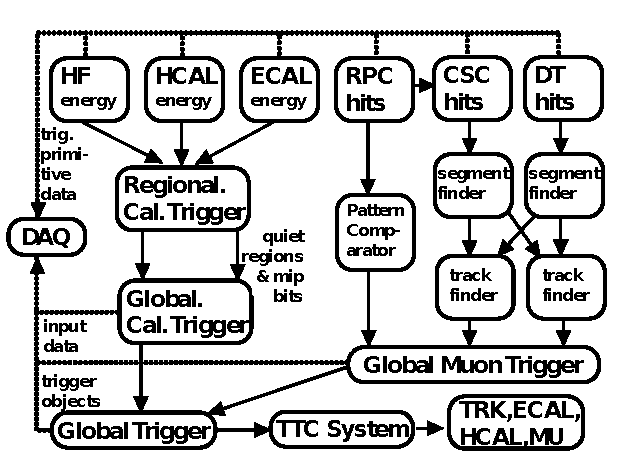
\includegraphics[width=0.7\textwidth]{figs/CMS-TRG-12-001_Figure_002.pdf}
\caption{The CMS L1 trigger system.}
\label{fig:l1}
\end{figure}
